\documentclass{article}
\usepackage[margin=24mm]{geometry}
\usepackage{tikz}
\usepackage[T1]{fontenc}
\begin{document}
\section*{Graph cross-platform measurement}
Created-at: 2026-09-06 12:50 +02:00.

\paragraph{Scope and acceptance} Execute the existing Graph search and algorithm clients on Windows, native Amaterasu and ARM64 Docker/QEMU on Amaterasu. Reuse canonical checkouts and target caches. Production and Cargo dependencies remain unchanged. Preserve checksums, correctness results, raw samples, median/IQR/worst, binary/source hashes and explicit unsupported metrics.
\paragraph{Workloads} Existing complete 48-cell informed Berge matrix: grids, weighted maps, corridor and transport; BFS/Dijkstra on path65k, grid256, STS1023, random1e6 and map512; bounded paths/cycles. Add existing reachability, components, rank-2 and Levi clients on path65k and STS511, plus independent 64-query batches at 1/2/4 threads on STS511. Rank-2 on non-rank-2 input remains explicitly not applicable. Three independent process runs per platform, two warmups and nine retained samples per cell. No representation expansion experiment is added.
\paragraph{Affected paths} scripts/performance\_evidence/campaign.py and test\_campaign.py; this plan bundle; reports/cross-platform-benchmarks/2026-09-06/* including raw logs, JSON/CSV and SVG; reports/2026-09-06-cross-platform-benchmarks.md; generated SYMBOLS.md only if required by the canonical index. Protected items touched: empty. No interface changes.
\paragraph{Tests} First validate parser against malformed rows, missing samples, drift and failures. Build pinned release clients and run their non-ignored correctness tests on all three platforms before timing. Compare invariant results and search work across runs/platforms; compare BFS and Dijkstra costs/hops, A* optimal costs. Unsupported CPU values remain missing, never zero. Source tree clean or explicitly recorded measurement-driver-only changes.
\paragraph{Budget and ETA} About 45--75 minutes: existing 48-cell baseline has 2 warmups plus 9 batches targeting 250ms each; three runs of 59 cells on three hosts, with local and remote campaigns on separate machines. QEMU does not run concurrently with native measurements or website builds. Compile four jobs, 16GiB memory cap; each process 180s timeout, report any overrun before changing scope. Stop on checksum drift or failure. Observe progress for every process and every ten seconds. No unbounded enumerations; existing max-depth/result/expansion limits stay authoritative.
\paragraph{Risks} Host noise, QEMU overhead, timer quantization and build interference. Record ambient CPU, exact compiler/lock/source/runtime image and excluded runs. Memory is whole-process peak, not per operation. Samples are batch means, not request tails. ARM results are emulated, not hardware claims.
\paragraph{Rollback} Revert campaign scripts/evidence commit, remove only named transient build staging after successful extraction, preserve reusable caches and all production sources.

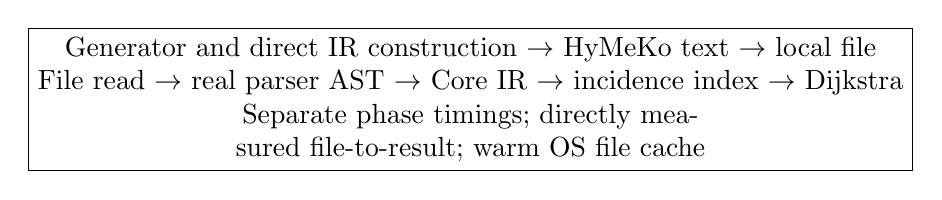
\begin{tikzpicture}\node[draw,text width=11cm,align=center]{Generator and direct IR construction $\to$ HyMeKo text $\to$ local file\\File read $\to$ real parser AST $\to$ Core IR $\to$ incidence index $\to$ Dijkstra\\Separate phase timings; directly measured file-to-result; warm OS file cache};\end{tikzpicture}


\section*{Parsing extension, created 2026-09-06 17:29 +02:00}
\paragraph{Ownership and discovery} Parser owns lexer/AST; Core owns interning,
resolution, lowering and ModuleStore; Graph owns the existing benchmark fixtures
and evidence campaign. The parser-backed ecoread repository and uses queries were
executed. Discovery: find parser benches, Graph informed clients and scripts;
grep parse/serialize/writer; read parser\_bench.rs, ir\_writer.rs,
ModuleStore, RealParser, informed\_common and statistics. Verdict: EXTEND the
Graph evidence client and campaign. IrWriter emits an arc placeholder and is not
a round-trip serializer; a private test fixture projection must preserve numeric
node annotations and signed weighted incidences and reject unsupported input.
No production serializer or parser is added. Baseline duplication: 517 clones,
12272 lines, 152 files. Fetch succeeded through the existing host's IP; integrate
fresh Graph main eae7a57 into the existing task branch, preserving previous data.
Core dependency remains locked to fc3eda9b; parser 284c490d.
\paragraph{Acceptance} Parse actual deterministic HyMeKo text for every distinct
source topology used by the existing 59 cells (query-distance variants share the
same source). Record source byte count and hash, nodes/arcs/incidences, correct
signed targets, weights and positions. Compare parsed IR with the generating IR
and check query reachability, optimal cost and valid path. Include explicit
parse rejection and corrupted fixture controls. Parser errors cannot count as
successful fast parses.
\paragraph{Phases} Measure resident UTF-8 text to AST; already parsed AST through
interning/resolution/lowering; complete fresh ModuleStore compilation (including
production validation and hashes); parsed IR to incidence index; and fresh
text through compilation/index/Dijkstra with a fresh workspace. Input generation,
filesystem I/O, strong verification and final object destruction stay outside
factory timings; intermediate pipeline destruction stays inside. End-to-end is
measured directly, never computed by adding medians. Reuse existing factory
sampling (2 warmups, 9 samples), resource telemetry and process driver. Three
fresh processes per cell per platform, sizes up to map512 and random1e6. Lexical
pattern suites already in parser remain separate from topology-specific rows.
\paragraph{Affected paths and authority} This existing plan bundle;
hymeko\_graph/tests/informed\_berge\_evidence.rs and new private
informed\_common/parsing.rs; scripts/performance\_evidence/campaign.py and its
tests; generated SYMBOLS.md; reports/2026-09-06-parsing-benchmarks.md and
reports/parsing-benchmarks/2026-09-06/* (CSV/JSON/logs/SVG/manifests).
The user's explicit request authorizes this benchmark-only test extension under
the protected Graph crate. No production edits or new dependencies. Website
reads the resulting Graph table using its existing generic adapter, at
/srv/apps/benchmark. No web source is placed in Core.
\paragraph{Budgets and ETA} Estimated 45--75 minutes including implementation,
focused tests, cached builds and three platform campaigns. Largest source is
map512 (262144 nodes, approximately 523000 arcs); nested AST and compiled stores
may consume much more memory than the original IR. Smoke largest inputs before
full runs; hard 16GiB RSS limit, 180 seconds per process initially. The new phase
wall costs are unknown: refine campaign ETA from the largest-input smoke before
launch, without reducing the declared matrix silently. Native and QEMU never
measure concurrently; no website build overlaps measurements. Reuse existing
checkouts, target caches, cross image and explicit QEMU on Amaterasu.
\paragraph{Rollback and interpretation} Revert only this benchmark extension;
keep original evidence immutable. Remove named transient deployment/build files
on completion. No worktrees/clones. Times characterize these pinned versions and
representations; serialized IR has edge declarations absent from the synthetic
IR and this overhead is reported. QEMU is emulation, not native ARM hardware.
This adds measurements, not a SOTA superiority claim.


\section*{Resource-bounded platform matrix, updated 18:07 +02:00}
The ARM64 map512 full-compilation smoke hit the declared 180-second process
budget (peak about 3.24GiB). It produced no accepted timing row. Do not expand
that optional full-frontend campaign into hours of emulation. The requested
parse timing remains mandatory on all 16 workloads and all three platforms.
Retain all five phases on Windows and native Amaterasu; run the parse\_ast phase
on ARM64, with the same source validation and unchanged Rust measurement binary.
Declared total: 240 Windows + 240 native + 48 ARM64 processes, 176 pooled rows.
Five-stage ARM64 coverage is explicitly incomplete, and the timed-out smoke is
retained as resource evidence, not converted to a latency value. Run the largest
parser-only ARM64 smoke before its full matrix. Driver phase selection is explicit
in provenance. A source-ref option is permitted only after Git proves the entire
Rust client, production Graph source and manifests/lock unchanged against that
reference; record the driver's separate revision and byte hash. Expected remaining
wall 20--35 minutes, revised after the parser-only ARM64 smoke. The existing
16GiB RSS and 180-second process budgets remain enforced.

The user's ongoing functional scope is Core, Graph, Transformation and Tensor,
with thin bindings in hymeko\_python where needed. Cross-repo capability discovery
is read-only while the pinned measurements complete. Preserve Transformation's
existing uncommitted geometry work. Tensor already owns seven Python numerical
bindings; do not duplicate them while planning a coherent Python surface.

\section*{Explicit phase breakdown, updated 2026-09-06 18:37 +02:00}
The user requests separate generation, graph construction, preparation, execution
and complete pipeline measurements, followed by publication to the existing website.
Extend the existing private SourceFixture and campaign, without production or
dependency changes. Existing generators construct IR directly: label this combined
operation generate\_ir, never claim a separately measured topology-only generation.
Add emit\_source (IR to text), read\_source (local UTF-8 file, warm OS cache),
dijkstra\_prepared (compiled IR and incidence index ready, fresh query workspace),
and file\_to\_dijkstra (read, compile, index, query). Keep existing five phases
and their evidence immutable. Temporary source-file writes and fixture validation
are outside all timed regions. File-to-result is measured directly, not summed.
No external-map importer is introduced in this benchmark-only change; import of
external road formats remains unmeasured. Test file read failure, byte equality,
generated IR equivalence, query result equivalence and each phase's nine samples.
Use 3 independent processes, 2 warmups and 9 samples. Windows measures only the
5 new phases; native measures the original and added phases in separate campaigns.
ARM64 retains all 16 parser-only cases; its full-compile timeout stays explicit.
Separate revision sets for old/new campaigns; no pooling across revisions.
Budget: 16GiB, 180 seconds per process. Smoke map512 and random1e6 first.
ETA 45--65 minutes: measured native original matrix about 15 minutes, added
phases about 15 minutes per native host, ARM64 parser-only about 15 minutes,
plus tests and website verification, with Windows independent of remote work.
Extend existing report, diagrams, campaign.py/test\_campaign.py and parsing.rs;
publish exact-byte CSV/JSON/SVG manifests under the existing evidence family.
Website is local-only Git at /srv/apps/benchmark (no remote configured); extend
its existing metric adapter, filters, table and tests to show stage and boundaries.
Run existing production build/tests and verify deployed API plus browser.
Graph f6bd760 is synchronized with its task upstream and contains current main.
Core checkout diverges from main but is read-only; Cargo.lock pins fc3eda9b.
Parser 284c490d is current. Preserve all other workers' files and prior evidence.
Rollback: scoped benchmark and website changes; retain original campaigns.
\end{document}
